\documentclass[12pt,a4paper]{article}
\usepackage[utf8]{vietnam}
\usepackage{amsmath,amssymb}
\usepackage{tabularx}
\usepackage{tikz}
\usepackage{xcolor}
\usepackage[top=0.6cm, bottom=0.6cm, left=0.6cm, right=0.6cm]{geometry}
\usepackage[dethi]{ex_test}

\SAOPTN{widthSA=2.6,heightSA=0.62}
\setlength{\parskip}{0pt}

% Dòng kẻ chấm mờ chuẩn viết tay
\newcommand{\dongke}[1]{%
  \begingroup%
  \setlength{\parskip}{0pt}%
  \baselineskip=18.5pt%
  \vspace{1.0mm}%
  \foreach \i in {1,...,#1}{%
    \noindent{\color{gray!60}\dotfill}\par%
  }%
  \vspace{0.6mm}%
  \endgroup%
}

% Khu vực bài làm chia 2 cột có vách ngăn mờ ở giữa
\newcommand{\dongkeHaiCot}[1]{%
  \par\vspace{0.5mm}%
  \noindent%
  \begin{minipage}[t]{0.485\linewidth}%
    \dongke{#1}%
  \end{minipage}%
  \hfill%
  {\color{gray!60}\vrule}%
  \hfill%
  \begin{minipage}[t]{0.485\linewidth}%
    \dongke{#1}%
  \end{minipage}%
}

% Định nghĩa ô bài tập tự luận trong bảng
\newcommand{\oBaiTap}[3][5]{%
  \vspace{1.0mm}%
  \noindent\textbf{#2} #3\par%
  \dongke{#1}%
}

\begin{document}
\pagestyle{empty}
% =============================================================================
% ========================= MA DE 05 - MAT TRUOC (TRANG 1/2) =============
% =============================================================================
\noindent
\begin{tabularx}{\linewidth}{|X|c|}
\hline
\textbf{PHIẾU KIỂM TRA ĐỊNH KỲ TOÁN 7 - TUẦN 12 - BUỔI 01} & \textbf{Mã đề: 05 - Trang 1/2} \\
\hline
\end{tabularx}

\vspace{1.0mm}

\noindent
\begin{tabularx}{\linewidth}{|p{3.2cm}|X|}
\hline
\centering\textbf{ĐIỂM SỐ} & \centering\textbf{LỜI NHẬN XÉT CỦA THẦY CÔ} \tabularnewline
\hline
\rule{0pt}{1.8cm} & \tabularnewline
\hline
\end{tabularx}

\vspace{1.2mm}
\noindent\textbf{Câu 1 (0,25 điểm).} Cho $\triangle ABC$ cân tại $A, \widehat{A} = 48^\circ$. Tính: $\widehat{B} =$ \shortans{66^\circ}\par\vspace{2.5mm}
\noindent\textbf{Câu 2 (0,25 điểm).} Cho $\triangle MNP$ cân tại $M, \widehat{N} = 68^\circ$. Tính: $\widehat{M} =$ \shortans{44^\circ}\par\vspace{2.5mm}
\noindent\textbf{Câu 3 (0,25 điểm).} Cho $\triangle ABC$ vuông cân tại $B$. Số đo góc $A$ là: \shortans{45^\circ}\par\vspace{2.5mm}
\noindent\textbf{Câu 4 (0,25 điểm).} Cho $\triangle ABC$ cân tại $B$ có $\widehat{B} = 60^\circ$. $\triangle ABC$ là tam giác gì? \shortans{Tam giác đều}\par\vspace{2.5mm}
\noindent\textbf{Câu 5 (0,25 điểm).} Cho $\triangle ABC$ cân tại $A, AB = 10\text{ cm}, BC = 6\text{ cm}$. Chu vi là: \shortans{26\text{ cm}}\par\vspace{2.5mm}
\noindent\textbf{Câu 6 (0,25 điểm).} Giá trị của $\sqrt{225} =$ \shortans{15}\par\vspace{2.5mm}
\noindent\textbf{Câu 7 (0,25 điểm).} Tính giá trị: $|-7{,}3| + |2{,}7| =$ \shortans{10}\par\vspace{2.5mm}
\noindent\textbf{Câu 8 (0,25 điểm).} Tính giá trị: $\left(-\dfrac{1}{4}\right)^3 =$ \shortans{-\dfrac{1}{64}}\par\vspace{2.5mm}
\noindent\textbf{Câu 9 (0,25 điểm).} Mái nhà hình tam giác cân có góc đỉnh $120^\circ$. Góc dốc của mái là: \shortans{30^\circ}\par\vspace{2.5mm}
\noindent\textbf{Câu 10 (0,25 điểm).} Cho $\triangle ABC$ có $\widehat{B} = 75^\circ, \widehat{C} = 30^\circ$. $\triangle ABC$ cân tại đâu? \shortans{Đỉnh C}\par\vspace{2.5mm}
\vspace{0.2mm}
\noindent\textbf{Câu 11 (3,0 điểm). Thực hiện phép tính (hợp lý nếu có thể):}
\vspace{0.5mm}

\noindent
\begin{tabularx}{\linewidth}{|X|X|}
\hline
\oBaiTap[5]{a) (0,5 điểm)}{$\dfrac{9}{14} + \left(-\dfrac{5}{11}\right) + \dfrac{5}{14} + \left(-\dfrac{6}{11}\right)$} & 
\oBaiTap[5]{b) (0,5 điểm)}{$\dfrac{8}{17} \cdot \left(-\dfrac{14}{23}\right) + \dfrac{8}{17} \cdot \left(-\dfrac{9}{23}\right)$} \\
\hline
\oBaiTap[5]{c) (0,5 điểm)}{$\sqrt{\dfrac{81}{25}} - \left(-\dfrac{1}{2}\right)^2 : \dfrac{5}{8}$} & 
\oBaiTap[5]{d) (0,5 điểm)}{$\dfrac{7}{10} - \left[\dfrac{1}{3} - \left(\dfrac{5}{6} - \dfrac{1}{2}\right)\right]$} \\
\hline
\oBaiTap[5]{e) (0,5 điểm)}{$\left|-\dfrac{4}{5}\right| : \dfrac{8}{5} + \sqrt{\dfrac{9}{16}} - 1{,}25$} & 
\oBaiTap[5]{f) (0,5 điểm)}{$\dfrac{8^3 \cdot 9^2}{2^8 \cdot 3^3}$} \\
\hline
\end{tabularx}

\newpage
% =============================================================================
% ========================= MA DE 05 - MAT SAU (TRANG 2/2) ==============
% =============================================================================
\noindent
\begin{tabularx}{\linewidth}{|X|}
\hline
\centering\textbf{TOÁN 7 - TUẦN 12 - BUỔI 01 | Mã đề: 05 - Trang 2/2} \\
\hline
\end{tabularx}

\vspace{1.2mm}

\noindent\textbf{Câu 12 (2,0 điểm). Tìm số hữu tỉ $x$, biết:}
\vspace{0.5mm}

\noindent
\begin{tabularx}{\linewidth}{|X|X|}
\hline
\oBaiTap[5]{a) (0,5 điểm)}{$x - \dfrac{5}{6} = -\dfrac{1}{3}$} & 
\oBaiTap[5]{b) (0,5 điểm)}{$\dfrac{2}{5}x + \dfrac{1}{3} = -\dfrac{7}{15}$} \\
\hline
\oBaiTap[5]{c) (0,5 điểm)}{$\left|x - \dfrac{1}{4}\right| = \dfrac{3}{4}$} & 
\oBaiTap[5]{d) (0,5 điểm)}{$\left(x + \dfrac{2}{3}\right)^2 = \dfrac{16}{9}$} \\
\hline
\end{tabularx}

\vspace{1.2mm}

\noindent
\begin{tabularx}{\linewidth}{|X|}
\hline
\vspace{0.5mm}
\begin{minipage}[t]{0.62\linewidth}
\vspace{0pt}
\textbf{Câu 13 (2,0 điểm).} Cho tam giác $ABC$ cân tại $A$ ($\widehat{A} < 90^\circ$). Gọi $D$ là trung điểm của cạnh $BC$.\par\vspace{0.3mm}
\textbf{a) (1,0 điểm)} Chứng minh $\triangle ABD = \triangle ACD$. Suy ra $AD \perp BC$ và $AD$ là phân giác $\widehat{BAC}$.\par\vspace{0.3mm}
\textbf{b) (1,0 điểm)} Từ $D$ kẻ $DH \perp AB$ ($H \in AB$), $DK \perp AC$ ($K \in AC$). Chứng minh $DH = DK$ và $\triangle DHK$ cân.
\end{minipage}\hfill
\begin{minipage}[t]{0.36\linewidth}
\vspace{0pt}\centering
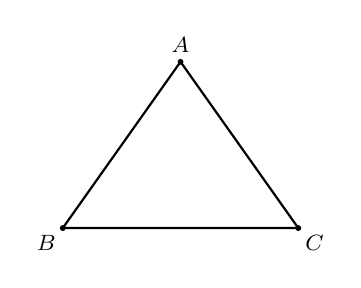
\begin{tikzpicture}[scale=0.88, line cap=round, line join=round, >=stealth, font=\footnotesize]
  \coordinate (A) at (0, 2.4);
  \coordinate (B) at (-1.7, 0);
  \coordinate (C) at (1.7, 0);

  \draw[thick] (A) -- (B) -- (C) -- cycle;

  \fill (A) circle (1.2pt) node[above] {$A$};
  \fill (B) circle (1.2pt) node[below left=-1pt] {$B$};
  \fill (C) circle (1.2pt) node[below right=-1pt] {$C$};
\end{tikzpicture}
\end{minipage}\par
\vspace{0.4mm}
\noindent\textit{Bài giải:}\dongkeHaiCot{10}
\\ \hline
\end{tabularx}

\vspace{1.2mm}

\noindent
\begin{tabularx}{\linewidth}{|X|}
\hline
\vspace{0.5mm}
\textbf{Câu 14 (0,5 điểm).} Tìm giá trị lớn nhất của biểu thức: $E = \dfrac{24}{|x - 5| + 6}$ với $x \in \mathbb{R}$.\par
\vspace{0.4mm}
\noindent\textit{Bài giải:}\dongkeHaiCot{6}
\\ \hline
\end{tabularx}
\end{document}
